%*----------- SLIDE -------------------------------------------------------------
\begin{frame}[c]{Processing}
    %\transboxin[duration=1,direction=30]
 
    \begin{itemize}
        \item Processing é uma linguagem de programação Open-Source e IDE (Ambiente de Desenvolvimento Integrado) construído para projetos visuais principalmente, e para servir como base de cadernos eletrônicos.
        \item É uma linguagem com grande assimilação às linguagens "C" e "Java", grandes inspirações da liguagem, resultando em algo que remete à programação em C com aspectos da programação orientada a objetos do Java.
    \end{itemize}
	\vspace{0.4cm}
	\centering
	
\includegraphics[width=0.3\textwidth]{processing-logo}   

%*----------- notes
    \note[item]{Notes can help you to remember important information. Turn on the notes option.}
\end{frame}
%-
%*----------- SLIDE -------------------------------------------------------------
\begin{frame}[t]{Arduino}
      \begin{itemize}
        \item Arduino é uma plataforma de prototipagem e hardware livre, projetado como um microcontrolador.
        \item Utilizando a liguagem C/C++ como base, o Arduino tornou-se bastante popular por apresentar baixo custo, flexibilidade e facilidade de manuseio em desenvolvimento de sistemas interativos.
    \end{itemize}
\vspace{0.3cm}
\begin{columns}
	% Column 1
	\begin{column}{0.4\textwidth}
        	\centering
		
\includegraphics[width=0.5\textwidth]{arduino-logo} 
	\end{column}
	% Column 2    
		\begin{column}{0.4\textwidth}
		\centering
       	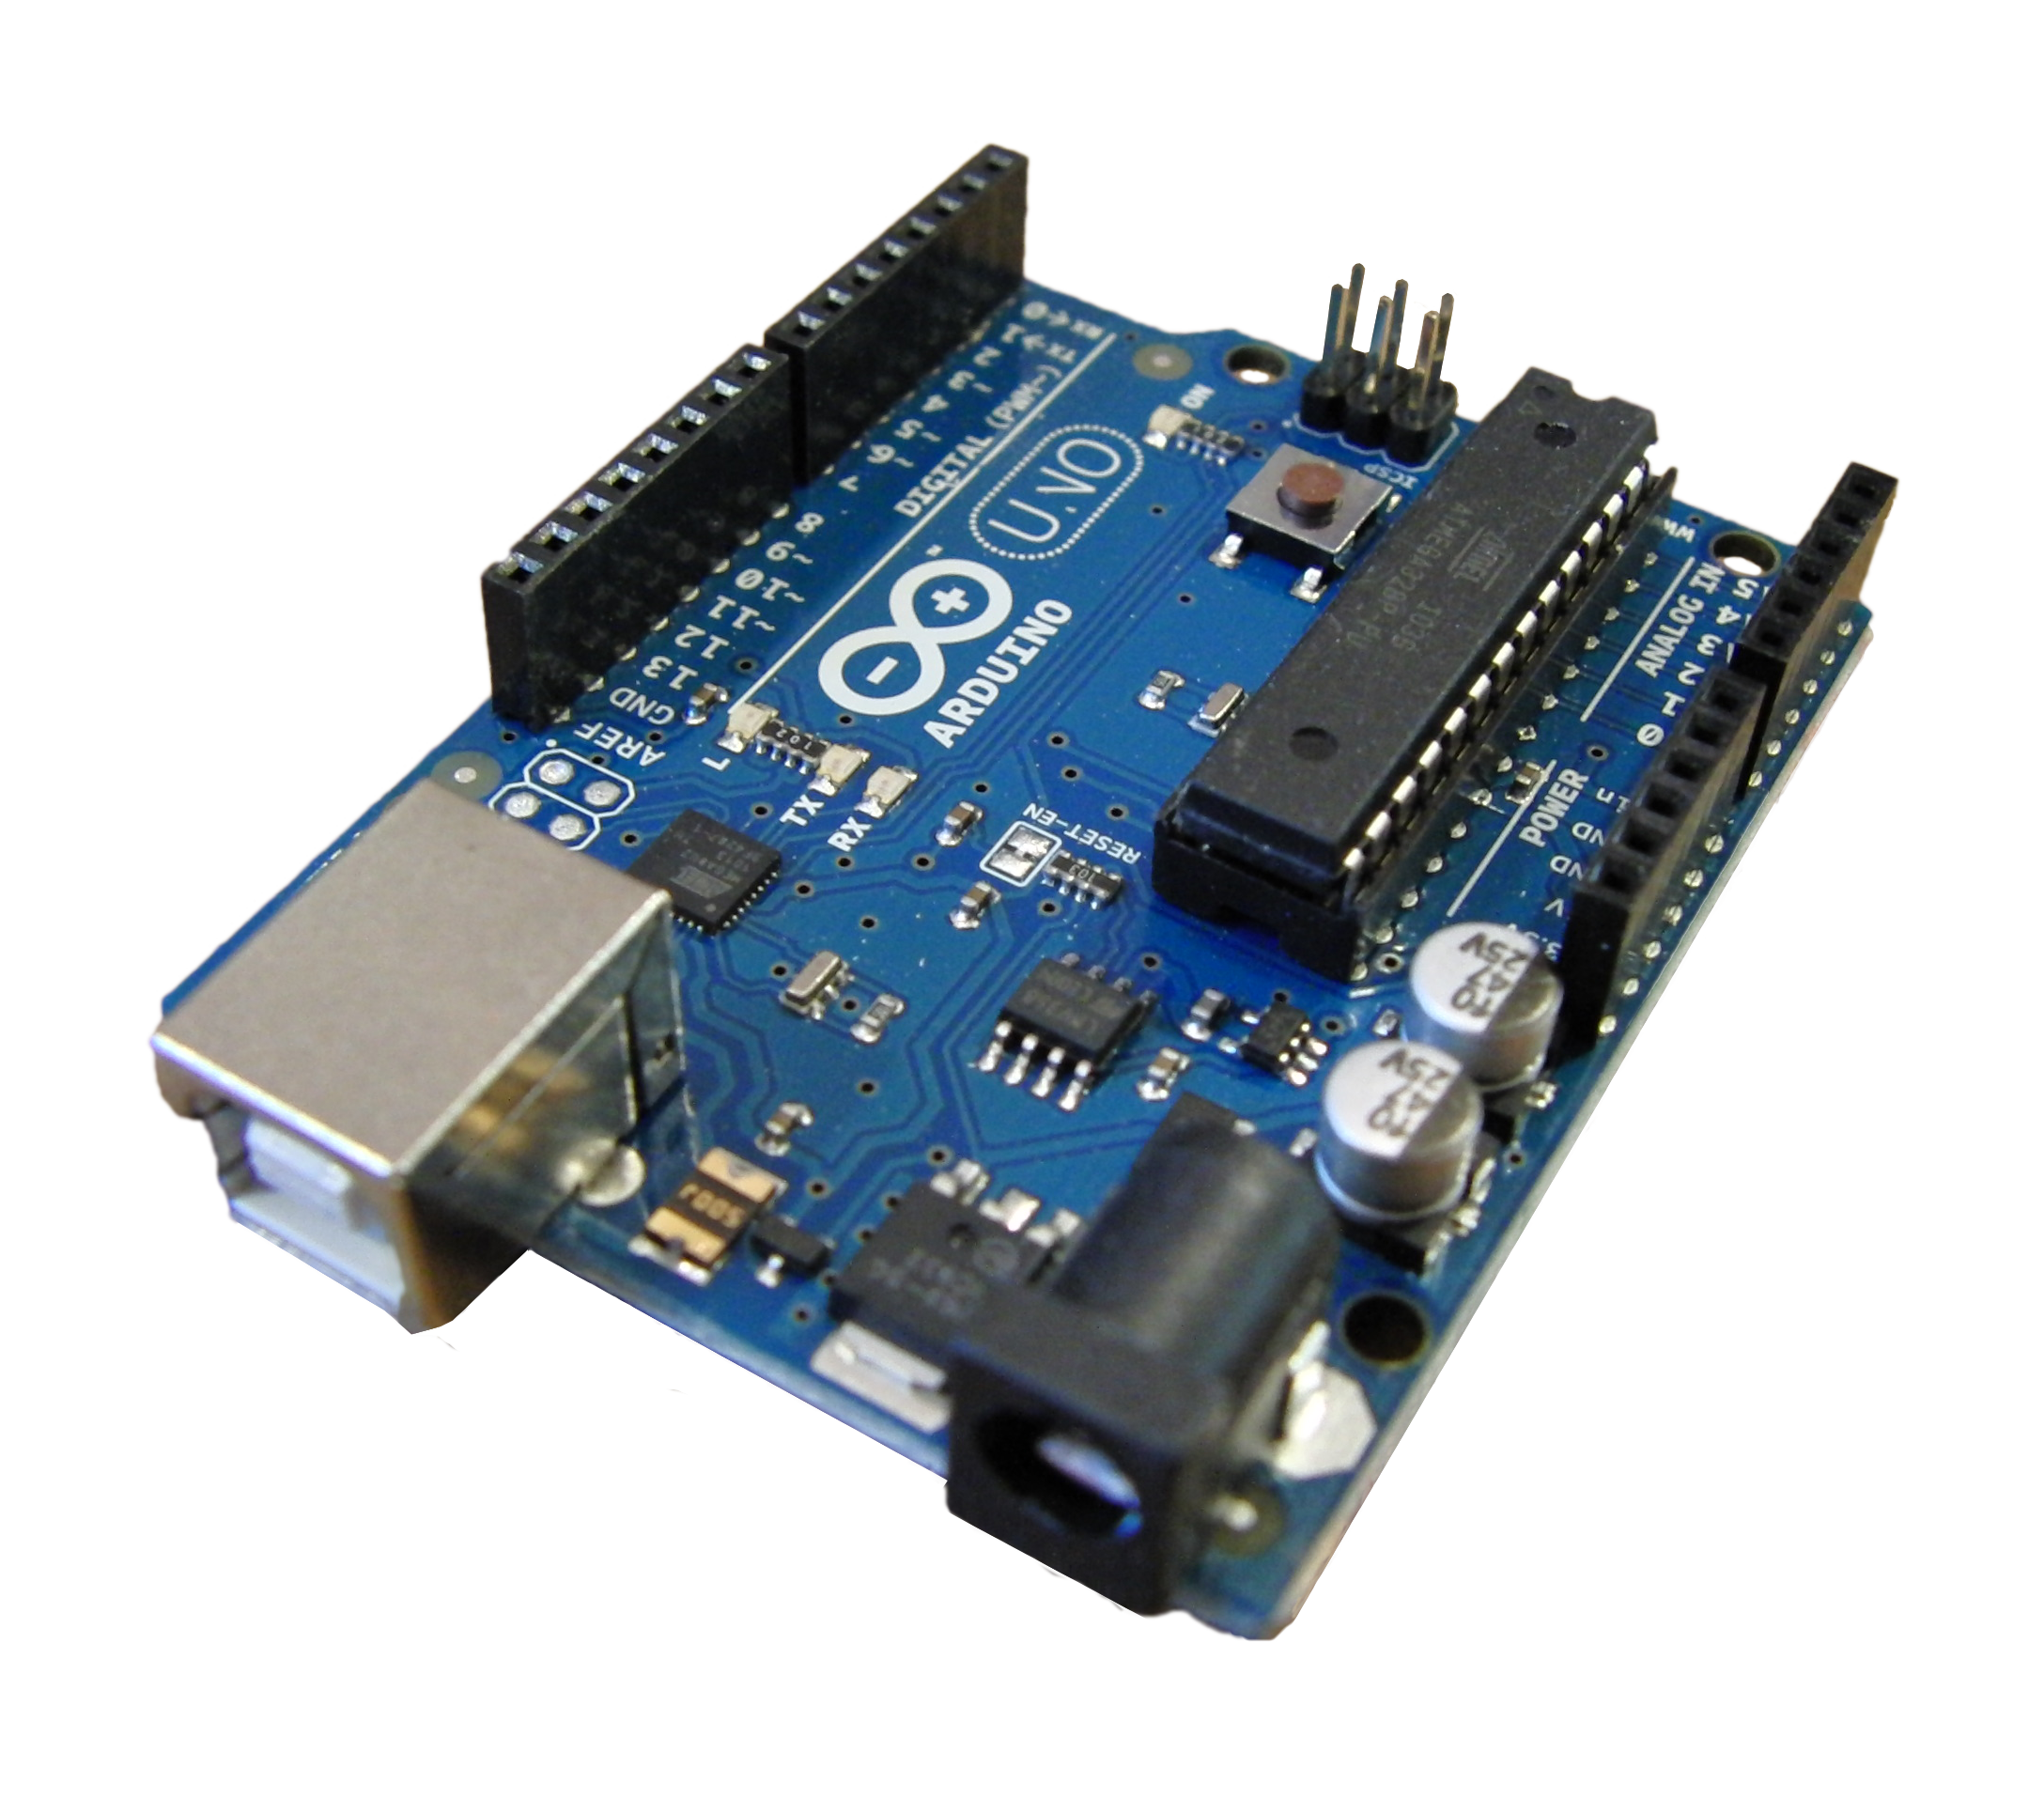
\includegraphics[width=0.7\textwidth]{arduino} 
	\end{column}
\end{columns}


%*----------- notes
    \note[item]{Notes can help you to remember important information. Turn on the notes option.}
\end{frame}
